\documentclass[10pt,a4paper]{article}
\usepackage[utf8]{inputenc}
\usepackage{amsmath}
\usepackage{amsfonts}
\usepackage{amssymb}
\usepackage{graphicx}
\usepackage[ngerman]{babel}
\usepackage[a4paper, portrait, margin=1.2in]{geometry}
\author{AW, TS, CS, AD, RB}
\title{Großes Studienprojekt}


\begin{document}
\maketitle
\begin{abstract}
  Da IPv4 aufgrund von immer weiter steigenden Nutzerzahlen
  und internetfähigen Geräte bald nicht mehr als
  Standardadressraum verwendet werden kann und IPv6 eine
  mögliche Lösung dieses Problems ist, haben wir uns innerhalb
  unseres großen Studienprojektes mit dem Aufsetzen und
  Verwalten eines IPv4 bzw. IPv6 Netzwerkes
  auseinandergesetzt.
\end{abstract}
\section{Fragestellung}
Um sich mit dem Zusammenspiel von Geräten innerhalb eines
Netzwerkes vertraut zu machen, war gefordert das folgende
Diagramm als Netzwerk umzusetzen:
\begin{figure}[ht]
  % 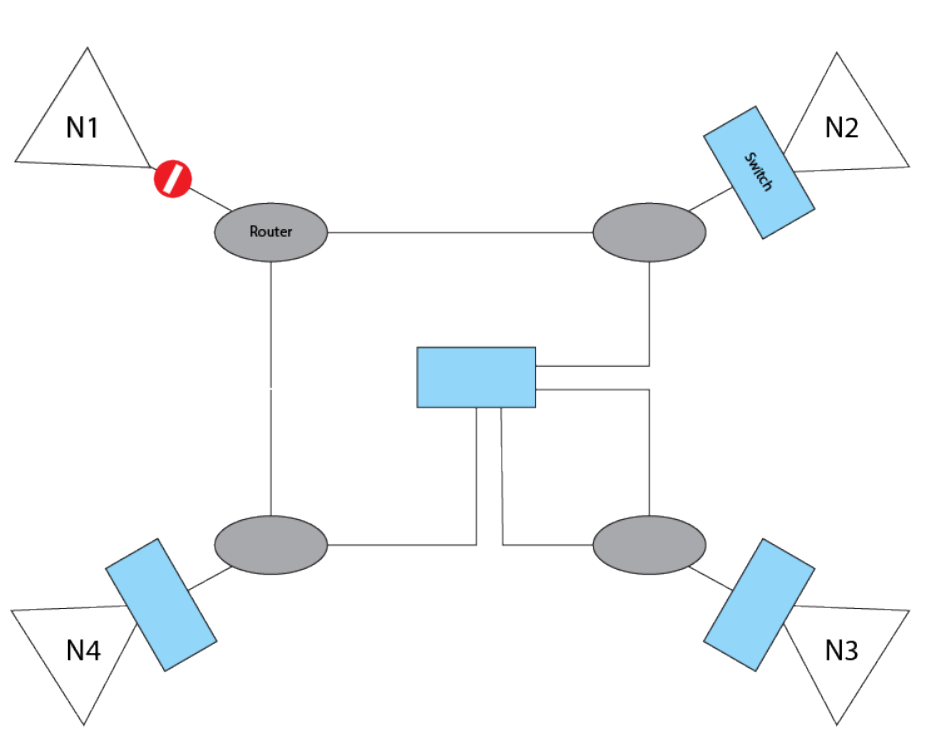
\includegraphics[width=\linewidth]{img/network_topography.png}
  \centering
  \caption{Aufbau des Netzwerks}
\end{figure}
\par
Die mit N1 bis N4 beschriftete Dreiecke bezeichnen die von uns
erstellten Subnetze, die durch die Router (graue Ovale, R1 bis R4)
verwaltet werden, und die blauen Vierecke repräsentieren jeweils einen
Switch. Das \glqq Einfahrt Verboten\grqq~ Schild symbolisiert
zusätzlich eine von uns konfigurierte Firewall.
\par
Jeder Router verwaltet die Vergabe der IPs innerhalb der eigenen
Subnetze über einen eigenen DHCP-Server. Alle Router erkennen sich und
kommunizieren untereinander über statische Routen, wobei die
Kommunikation zwischen R2 und R4 zwei Hops (über R1) benötigt.
Außerdem werden die Verbindungen zwischen R2 und R3, und R3 und R4
über einem Switch und durch zwei unabhängige VLANs realisiert, die
über den Switch in der Mitte konfiguriert werden.
\par
Hinter R1 ist eine Verbindung zum Internet, die durch die Firewall
geschützt wird, welche durch den Gebrauch von \texttt{iptables}
realisiert wurde. Die Firewall ist so konfiguriert, dass sie den
ausgehenden Verkehr nicht einschränkt, jedoch eingehende Pakete
weiterleitet, wenn sie im Zusammenhang mit ausgehenden Paketen stehen.
\par
Der innere Switch sollte zusätzlich so konfiguriert sein das er die
Verbindungen zu den Routern über die verbliebene Ports spiegelt.

\section{Herangehensweise}
Nach ersten Recherchen bezüglich der Router und deren Funktionsweise
fiel uns auf, dass diese mit einer veralteten Firmwareversion
ausgestattet waren. Deshalb war der erste Arbeitsschritt das
Aktualisieren der Firmware. Die jetzt aktualisierte Firmware verfügte
über eine GUI, mit deren Hilfe jegliche Einstellungen bezüglich der
IPv4-Einstellungen konfiguriert werden konnten.
\par
Bevor die Aufgabe bearbeitet wurde war eine Einarbeitung in die
Funktionen und Eigenschaften des Systems erforderlich, um eine
vollständige Umsetzung der Fragestellung zu realisieren. Dazu wurde
ein simples Netzwerk mit Hilfe der Konsole konfiguriert. In diesem
Netzwerk wurden alle für die Aufgabenstellung wichtige
Komponenten (z.B. DHCP, Firewall, Static Routes, usw.) eingebunden, um
ein tieferes Verständnis dieser zu gewinnen.
\par
Nach ersten Konfigurationen wurde mit Hilfe der GUI geprüft, ob alle
Einstellungen erfolgreich übernommen wurden. Weil das Konfigurieren
der Router über die GUI deutlich einfacher und übersichtlicher ist,
wurde zur Umsetzung der Aufgabenstellung eine Kombination aus Konsole
und GUI verwendet.
\par
Bei der Bearbeitung der Aufgabe musste zu aller erst das Netzwerk auf
physischer Ebene, wie auf Abbildung 1 zu sehen, zusammengesetzt
werden. Dabei war eine übersichtliche Verkabelung wichtig, um die
Subnetze auch unproblematisch unterscheiden und visualisieren zu
können. Des Weiteren wurden die Router etikettiert um weitere
Übersicht und Organisation zu erschaffen.
\par
Wichtig war die Dokumentation des Verlaufs der Umsetzung, als auch
eine Möglichkeit ältere Konfigurationen zu sichern und wieder
herzustellen. Hierzu wurde Git auf dem berühmten Hostingplattform
Github verwendet, dies erlaubte eine bessere Organisation des Projekts
und effektivere Zusammenarbeit.


\section{Konfiguration}Christopher


\section{Netzwerkanalyse}
Um die realisierte Topologie zu auf Richtigkeit überprüfen, wurde nach
der Konfiguration sowohl die Erreichbarkeit unter den einzelnen
Geräten, als auch die Verbindungsrouten selbst mit Hilfe verschiedener
Methoden getestet.
\par
Für die Erreichbarkeit zu bewerten, wurden zunächst Ping-Tests
veranlasst, welche jeweils von einem Gerät an einem Spezifischem
Router zu einem Gerät, welches an einem anderem Router angebunden
war. Um zu verhindern, dass ein falsches Gerät versucht wird zu
erreichen, haben wir uns zunächst die einzelnen IP-Adressen der
jeweiligen Rechner mit dem Konsolen-Befehl \texttt{ifconfig} beschafft. Die
Tests verliefen alle erfolgreich, was uns dazu führte, das Netzwerk
weitergehend zu untersuchen.
\par 
Bevor wir jedoch TCP oder UDP basierende Pakete über die internen
Leitungen versendet haben, richteten wird zunächst einen
bereitgestellten Rasberry-Pi ein, sodass dieser einen SSH-Server zur
verfügung stellte, jener dazu benutzt wurde um SSH und sftp-Anfragen
zu realisieren. Um weitergehende Informationen zu erhalten, wurde ein
dritter Rechner (A1) am Mirror-Port des Switches mit den VLANs
eingebunden, dieser mit Wireshark die Verbindungen und Übertragungen
analysierte.
\par
Die Verbindung über Ping(ICMP), ssh oder auch sftp von R1 nach R3
verursachte bei A1 keinen angezeigten Datenverkehr, was zu erwarten
war, dar die Router 0, 1 und 3 über Static Routes verbunden sind und
somit das Routing und der Datenaustausch über jene abgewickelt wurden.
\par
Alle anderen Verbindungen, welche über oder mit R2 hergestellt wurden
zeigten bei den jeweiligen Tests die zu erwartenden Protokolle an. Bei
den Ping-Tests kam das ICMP-Protokoll zum tragen. Bei den SSH und SFTP
Verbindungen wurde TCP und SSH verwendet, jedoch war die Gewichtung
der einzelnen Pakete unterschiedlich. So war die Paketverteilung von
SSH zu TCP beim SSH-Test ungefähr 2 zu 1, wohingegen beim SFTP-Test
der Anteil an SSH Paketen wesentlich höher war.


\section{Evaluation}Thomas
\end{document}